
In the following paragraphs I will describe the three measures of complexity I used in here: relative area/volume, disparity and roughness. I consider them complexity measures because they inform about specific features in embryonic development that are intuitively associated to the increasing complexity of the organism. The relative area/volume of expression relates to the notion of the progressive compartmentalization of the embryo, disparity informs about how the different parts of the embryo become more different (at the genetic level) from each other, and the roughness measure relates to the notion of genes being expressed in progressively more complex spatial expression patterns (as defined by the shape of the gene expression pattern).  For information on the statistical tests used (e.g., Kruskal Wallis, ANOVA, permutation test) see the corresponding study.


\subsubsection{Compartmentalization}

As mentioned before, the process of embryo compartmentalization, is expected to be largely reflected in the expression of the genes in progressively smaller areas. Therefore, a good measure of compartmentalization would be to measure the relative area of expression of all genes during development.
Gene expression patterns are usually visualized as 2D images, which reflect the distribution of a gene product from a specific anatomical view (e.g., lateral, dorsal).  Recently, methods like 3D imaging technique Optical Projection Tomography  \citep{Sharpe2003,Summerhurst2008} allow to record gene expression patterns in 3D.
%
In the case of 2D images, the measure of compartmentalization I use in here is the relative area of the expression, i.e., the pixels with expression divided by all the pixels of the embryo image. This "relative area" measure ranges from 0 (no expression) to 1 (ubiquitous expression). 
In the case of a gene expression in 3D, the compartmentalization measure becomes the relative volume of expression, which also ranges from 0 to 1 and is calculated as the volume of the cells/tissues with expression divided by the whole embryo volume.
%Of course it could be said that the compartmentalization of an embryo should not only be reflected in the decrease of the relative area of expression of the genes during development, but also should be reflected in a greater proportion of genes expressed differentially in different parts of the embryo. To account for this, I used a "disparity" measure (explained below), that would be informative in the mean degree of dissimilarity between the different parts of the embryo.

\subsubsection{Disparity}

The disparity measure is related to  McShea's "number of part types" complexity measure. Ideally, the number of cell types, if this could be precisely known, would be a good measure of complexity during development. However, as mentioned before, there is no clear criteria to determine when (at the genetic level) a new cell type is formed during development.
%
%Usually, genetic markers are used to determine if a cell (or its descendants) can be considered a specific cell type. This could be the case of anterior or posterior compartment cells within \textit{D. melanogaster} para-segments. For example, the use of wingless (\textit{wg}) or sonic hedgehog (\textit{hh}) in situ hybridization can be used to define if a cell is part of the anterior or posterior compartment. It could be said, however, that the earliest presence of expression of these genes marks the \textit{fate} of the cell, more than the actual cell type. In fact, before the anterior and posterior segment compartments are completely defined, the expression level of these genes changes over time and form a positive feedback to stabilize each other expression. Therefore, a cell that early expresses \textit{wg} would not necessarily differentiate into a posterior compartment if its neighbour para-segment does not express \textit{hh} \citep{Bejsovec1991}.
%
Instead of trying to determine the number of cell types during development, I decided to quantify how different at the gene expression level are the cells or regions in the embryo. In \textit{D. melanogaster}, as it was not possible to have expression for each individual cell, I divided the 2D embryo in "regions" of approximately the same area using polar coordinates (Fig. \ref{fig:roughness_regions}A; see study I). 
In the case of \textit{C. intestinalis}, I used expression data at a single cell level for the early stages and at tissue level for the tailbud stages (see study II).

To quantify this, I decided to use pearson's correlation as similarity measure between cells/tissues or regions. With this method, the expression of all the genes available in two cells can be compared, giving a value of 1 if all genes have exactly the same expression (their expression is completely correlated), to -1 if all the genes show opposite gene expression (their expression is anti-correlated). 
An advantage of this method is the possibility to include the information of all available genes, diminishing a possible bias in the gene selection. 
%
%The pearson's correlation matrix is a measure of gene expression similarity between genes. 
I computed pairwise similarities between cells/regions as the Pearson correlations using the function \textit{corSimMat} of the R package \textit{apcluster} \citep{Bodenhofer2011}. In here, I was interested on quantifying the difference (i.e., disparity) in gene expression between cells, not on their similarity. Therefore, the disparity between two cells becomes: disparity = 1 - pearson's similarity. The disparity measure ranges from 0 to 2, with a 0 value when the gene expression between cells is exactly the same.

\paragraph{Synexpression Territories} 
%Another advantage of using a Pearson's correlation matrix, is the possibility of using a clustering algorithm (e.g., hierarchical clustering). This has been used, for example, to find the main temporal patterns of gene expression in microarray analysis \citep{Eisen1998,Wen1998}.

Using the Pearson's similarity matrix I performed a hierarchical clustering of cells/ regions using the function \textit{hclust} of the R package \textit{stats} \citep{RCoreTeam2014} with the average method UPGMA and an euclidean distance function. The resulting dendrograms, with as many terminal branches as cell/regions analysed, were cut into a given number of clusters, called in here "synexpression territories".
In \textit{D. melanogaster} (study I and III) the dendrogram resulting from the analysis of the regions of all stages was cut into 40 synexpression territories. The territories are not exactly the same between study I and III, as in study III the clustering was done again with the 1199 genes dataset (see section \ref{insitu_drosophila}).
In \textit{C. intestinalis} (study II), because the information in the early stages is at the cell level while in the tailbud is at the tissue level, we performed two separate synexpression territory analyses one with the 32, 64 and 112 cells stages (n = 1550 genes), and another one with the early, mid and late tailbud stages (n = 820 genes).
The dendrograms resulting from the early and tailbud stages were cut in 24 and 10 "synexpression territories".

%Also, this method can be used to separate cell types based on the genetic differences between them \citep{gohlmann2009gene}.
%\textbf{AQUI PONER LOS TERRITORIOS DE CIONA Y DROSOPHILA}

%%%%%%%%%%%%%%%%%%%%%%%%%%%%%%%%%%%%%%%%%%%%%%%%%%%%%%%%%%%%%%%%%%%%%%%%%%%%%%%%%%%%%%
\begin{figure}[h]
  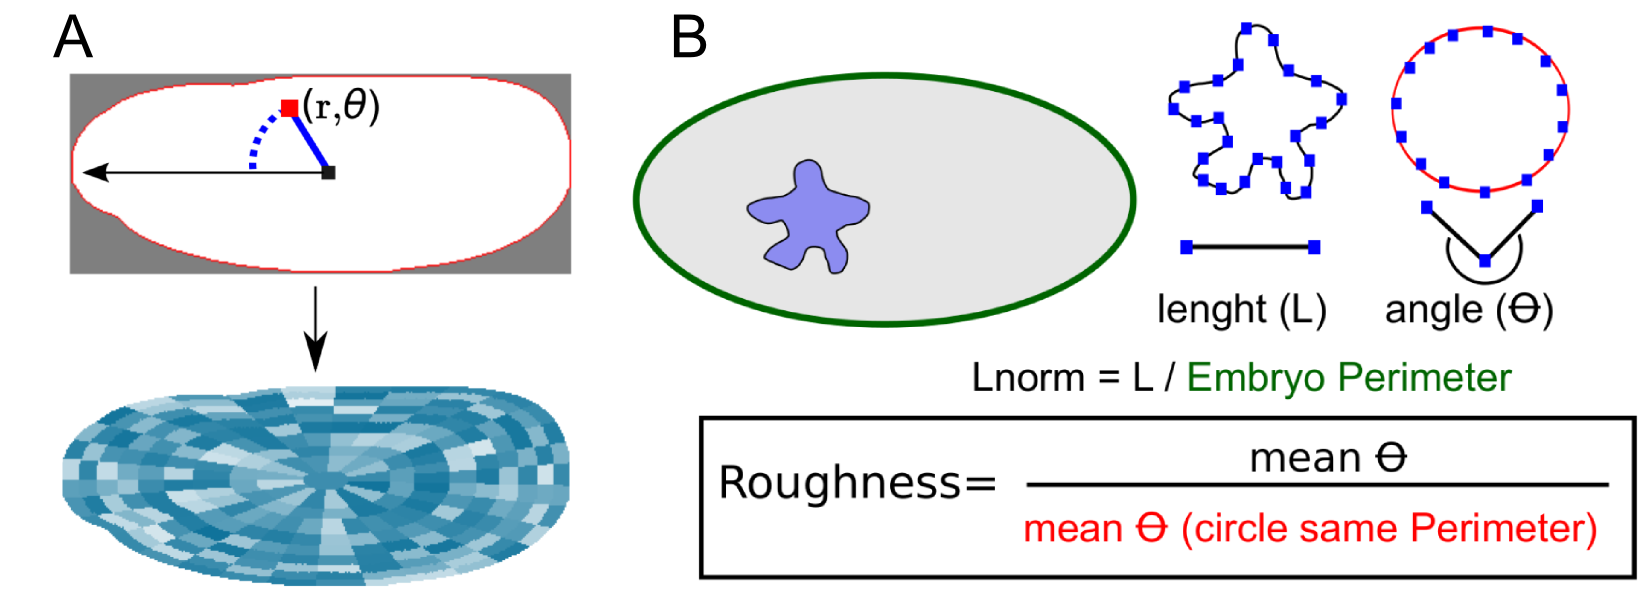
\includegraphics[width=0.75\textwidth]{./Images/roughness_regions.png}
  \centering
  \caption{\textbf{Polar regions and 2D roughness measure}. A) The embryo of each stage was divided in 257 regions using polar coordinates. The embryo for stage 11-12 is shown with the 257 regions in a random color. B) A schematic embryo (gray) with a gene expression pattern in blue. Roughness is the mean major angle ($\theta$) between each node (at every L length pixels in the contour) and its two immediate neighbours, normalized by the mean angle of a circle of the same perimeter. Image modified from Study I, reused with permission of Elsevier.
   }
  \label{fig:roughness_regions}
\end{figure}
%%%%%%%%%%%%%%%%%%%%%%%%%%%%%%%%%%%%%%%%%%%%%%%%%%%%%%%%%%%%%%%%%%%%%%%%%%%%%%%%%%%%%

\subsubsection{Roughness}
\label{Methods_roughness}
The roughness measure analyses the complexity of the shape of a gene expression pattern. In the case of 2D images, the shape of the gene expression pattern is extracted as a closed outline formed by the boundaries of gene expression. For 3D patterns, the shape of the expression pattern is the 3D external surface of the union of the cells that are expressing such gene.

Therefore, a gene expression pattern reflects necessarily the spatial distribution of the cells expressing such gene. When analysing and comparing the shape of diverse gene expression patterns, i.e., the cells/tissues with expression are different between genes, there is an obvious impossibility to determine landmark points (whether around a 2D outline or 3D surface) that would establish a clear one-to-one correspondence between them. This could be done in the case of comparing the expression pattern of a single gene at a specific developmental stage between different individuals.
Therefore, a landmark-free method (like outline methods for 2D or surface methods for 3D data) is best suited to deal with the type of data analysed in here.

There are practically no studies in the literature that have quantified and compared the shape of gene expression patterns in a systematic manner (one exception is the recent study of \citealp{Martinez-Abadias2016}). In here, I will consider that a gene expression pattern is complex based on the curvature of its 2D contour or 3D surface.

\paragraph{2D Roughness}
For 2D gene expression patterns, I used a "roughness measure", that is similar to the shape function $\phi^{*}(l)$ used in eigenshape analyses \citep{Lohmann1983}, as it measures how much the curvature of a closed outline deviates from the angles of a circle of the same perimeter (Fig. \ref{fig:roughness_regions}B; see study I). 
To calculate the roughness of a expression pattern I first selected points in the contour every L (length) pixels. Then, vectors between each node and the two immediate neighbour nodes in the contour are calculated and the biggest angle formed between them is measured. The roughness value is then the mean angle normalized by the mean angle of a circle of the same perimeter.

I selected the roughness measure instead of some other measure outline based method like Fourier analysis because the roughness value gives an intuitive descriptor of complexity, i.e., a value of 1 would be a simple "circle-like" shape, and a value greater than 1 would mean a higher curvature of the outline. \citet{McLellan1998} compared various measures of spatial complexity applied to the outlines of the leaves of many tree species. They included a "margin roughness" measure that is very similar to the one I use here (the difference is that they does not normalize by the mean angle of the circle nor he uses different lengths of vectors) and found that there was no marked differences between the margin roughness and a Fourier analysis with up to 64 harmonics (both performed equally well).
%On the contrary, one advantage of the Fourier analysis would be that it is an information preserving algorithm \citep{Pavlidis1980} i.e., it is possible to reconstruct the shape after the analysis, a feature that was not considered relevant for this study. 
Other feature of the roughness measure is that allows to measure the complexity of shape at different spatial scales (varying the L length). 
%Therefore, it can be tested not only if the complexity of the gene expression shape increases during development, also if this increase is the same at different spatial scales.

\paragraph{Dirichlet Normal Energy (DNE)}
	\nomenclature{DNE}{Dirichlet Normal Energy}
In order to use a similar measure of curvature in 3D, I used the Dirichlet normal energy (DNE; described briefly in section \ref{DNE_explanation}) which quantifies the deviation of a surface from being planar (Fig. \ref{fig:DNE}; see study II). 
Importantly, both measures are normalized to remove size and orientation effects.

%%%%%%%%%%%%%%%%%%%%%%%%%%%%%%%%%%%%%%%%%%%%%%%%%%%%%%%%%%%%%%%%%%%%%%%%%%%%%%%%%%%%%%
\begin{figure}[h]
  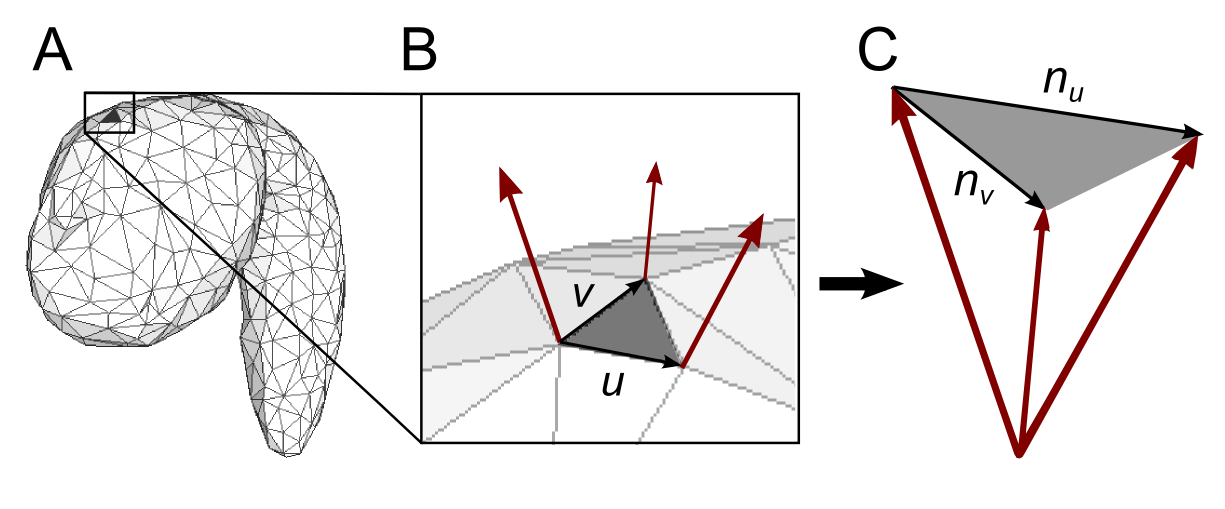
\includegraphics[width=0.6\textwidth]{./Images/DNE.png}
  \centering
  \caption{\textbf{Dirichlet Normal Energy (DNE).} A) A surface mesh representing a a mid-tailbud embryo in \textit{C. intestinalis}. B) DNE calculates the energy value $e(p)$ of each polygon (like the one in grey) in the surface. The polygon is characterized by vectors $u$ and $v$, which represent the edges of the polygon. Then, normal unit vectors are estimated as the normalized average of normal vectors of the triangle faces adjacent to each vertex (red arrows). C) If vertex normals are translated to a common origin point, their end points form a polygon with edge vectors $nu$ and $nv$, which represent the spreading of $nu$ and $nv$. In a simplistic way, DNE can be defined as the spreading of $nu$ and $nv$ relative to the spreading of $u$ and $v$  \citep{Bunn2011,Winchester2016}.
 }
  \label{fig:DNE}
\end{figure}
%%%%%%%%%%%%%%%%%%%%%%%%%%%%%%%%%%%%%%%%%%%%%%%%%%%%%%%%%%%%%%%%%%%%%%%%%%%%%%%%%%%%%

To calculate the DNE, I used the Morphotester software version 1.1.2 \citep{Winchester2016}
available in the webpage "http://morphotester.apotropa.com/". For details see study II.

It is important to mention that the aim of this analysis is not to discern which mechanisms (e.g., cell-cell signalling or morphogenetic movements) are responsible for the changes in complexity of the shape of gene expression pattern, but to quantify how this happens during embryonic development.

\subsubsection{The relationship between these measures}
\label{measures_relations}

The three different measures of complexity are informative of different and independent aspects of complexity and are not necessarily correlated. 
For example, a decrease in the area/volume of gene expression should not necessarily mean an increase in disparity, as the genes that are reducing their expression area could be restricted to the same part of the developing embryo. 
Only in the case of an embryo with all genes showing ubiquitous expression, there is a clear relationship between disparity and relative area/volume, as the relative area of expression and disparity would be 0 and 1 respectively. If there are however, many genes expressed in only a part of the embryo, these measures are not necessarily correlated. 

This can be illustrated with a simple example shown in Fig. \ref{fig:measures_relations}, in which there are different alternative gene expression scenarios of an imaginary embryo with six cells. In each scenario, the embryo expresses four genes in different relative areas (i.e., in a different number of cells). The mean relative area is 0.5 for all scenarios, but the mean disparity varies in a two-fold manner. In the scenario that shows the largest disparity, each cell expresses a unique combination of genes, while the scenario with the lowest disparity, 4 of 6 cells do not have a unique expression profile.

The roughness and disparity independence can be easily exemplified in the case of a blastula. Blastula is the name to define the multicellular aggregate stage that results from the subdivision (cleavage) of the zygote. The blastula shape topology and geometry is usually simple \citep{Forgacs_Newman2005}, typically consisting of a ball of cells with an interior cavity (called "blastocoel"). If in a spheric blastula, composed of also spheric cells (like that of a sea urchin) a large proportion of genes would be expressed ubiquitously and a small proportion of genes would be expressed in single cells, both roughness and disparity would be relatively low.
However in the case of a large proportion of genes expressed in different single cells, and a low proportion of genes expressed ubiquitously, the disparity would be high, but the roughness would be very similar than in the previous case. This would be because the roughness quantifies the shape of the expression pattern, irrespective to size. Therefore the roughness of a gene expression in a single spheric cell would be practically the same that the roughness of a gene expression in the whole spheric embryo.

The independence of the roughness measure with the size of the gene expression (i.e., relative area/expression) comes from the roughness normalization. The normalization of the 2D roughness consists of dividing the mean angle of a gene expression pattern by the mean angle of a circle with the same perimeter, and in the case of 3D roughness (i.e., DNE) it consists on transforming the 3D expression surface into a polygonal surface mesh with a determined number of polygons. 
%Therefore, these three measures of complexity should be informative on how genes become restricted to smaller regions (relative area/volume), how different is the gene expression of the different parts of the embryo (disparity) and how complex is the gene expression pattern shape (roughness) at different times of development.


%%%%%%%%%%%%%%%%%%%%%%%%%%%%%%%%%%%%%%%%%%%%%%%%%%%%%%%%%%%%%%%%%%%%%%%%%%%%%%%%%%%%%%
\begin{figure}[h]
  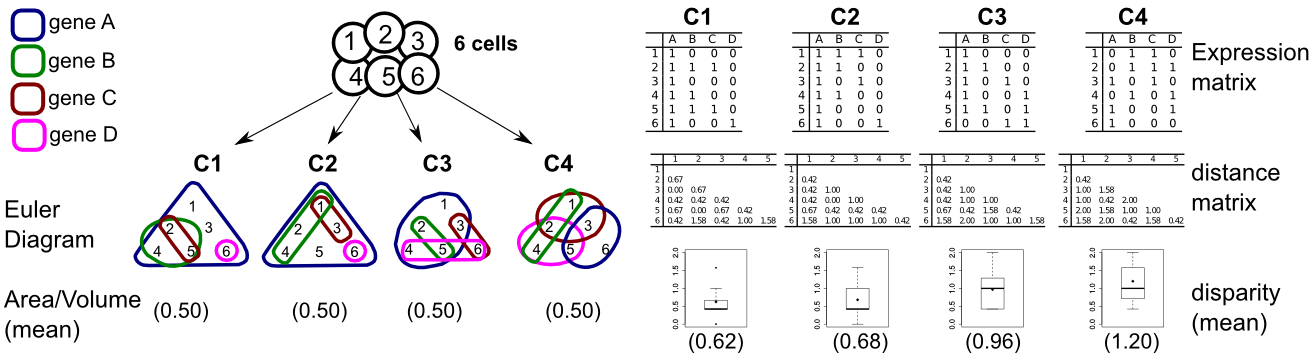
\includegraphics[width=0.95\textwidth]{./Images/measures_relations.png}
  \centering
  \caption{\textbf{Relation between area/volume of expression and disparity measures.} An embryo of six cells (top left) is shown expressing four different gene expression combinations (C1, C2, C3 and C4) of four genes (A, B, C and D). All combinations have a mean relative area/volume of 0.5. Each gene expression configuration is represented as an Euler diagram (representing the subset of the cells in which it is expressed in a color code shown at the top left) and as binary expression matrix (top right). The pairwise distance between the cells, calculated as 1-(pearson's correlation), is shown as a matrix. At the bottom right, a distribution plot of the pairwise distances of each combination and the mean disparity are shown below in parenthesis.
 }
  \label{fig:measures_relations}
\end{figure}
%%%%%%%%%%%%%%%%%%%%%%%%%%%%%%%%%%%%%%%%%%%%%%%%%%%%%%%%%%%%%%%%%%%%%%%%%%%%%%%%%%%%%
